\documentclass[../../main.tex]{subfiles}

 \lhead{Further Work}
 
\begin{document}

\section{Further Work}
\label{furtherwork}
	
	\subsection{Software}
		\subsubsection{Storage}
			%Not using Different RIR Grids but doing it in Max instead (Saving storage space)
			An issue with using the direct \ac{RIR} rendering method as stated in \cite{Savioja1999} is the storage required for the grid of \ac{RIR}'s. For this project, multiple grids were produced by taking the large grid of \ac{RIR}'s, extracting and storing the appropriate ones in separate files. This meant that a number of duplicate files were having to be stored. If time had allowed, a system in Max would have been designed to do the file extracting in real time, therefore requiring only one group of \ac{RIR} files as opposed to five. 

		\subsubsection{Iteration 1 Redesign}
			The failure to implement the desired \ac{RIR} interpolation method in the software used in this project has been noted several times, mentioning the system speed as being the culprit. As this design is more desirable than the one currently implemented, further work on the original design would be encouraged.

			One possible improvement could be to simplify the grid used for interpolation. Figure~\ref{grids} illustrates three implementations; \textbf{Grid 1} shows the layout of the original grid used where the user can move freely within the grid of RIRs. \textbf{Grid 2} shows a layout where only the \ac{RIR} locations at 90 degree increments to the user are available reducing the area in which the user can move (shown by the grey square). \textbf{Grid 3} shows a similar layout but using the \ac{RIR} locations at diagonals to the user. This would increase the area in which the user could move, however it would provide a less accurate approximation for the users position as the \ac{RIR}'s are more spread out.

			Another possibility in producing a faster running system could be to redesign the software in a more efficient programming language such as C++. This also has the potential to reduce system latency, thus reducing the amount of time needed to be cut off the beginning of the \ac{RIR}. This would in turn potentially avoid having to trim the direct wall reflections of a number of \ac{RIR} files.

		\subsubsection{UI cross platform}
			As the design in the Max patch enables the user interface to be resized for any type of screen while still maintaining the correct ratio of \ac{RIR} placements, it would be nice to see the user interface implemented on a less obtrusive device, allowing the user to change their location on their smartphone.

			\begin{figure}[H]
				\centerline{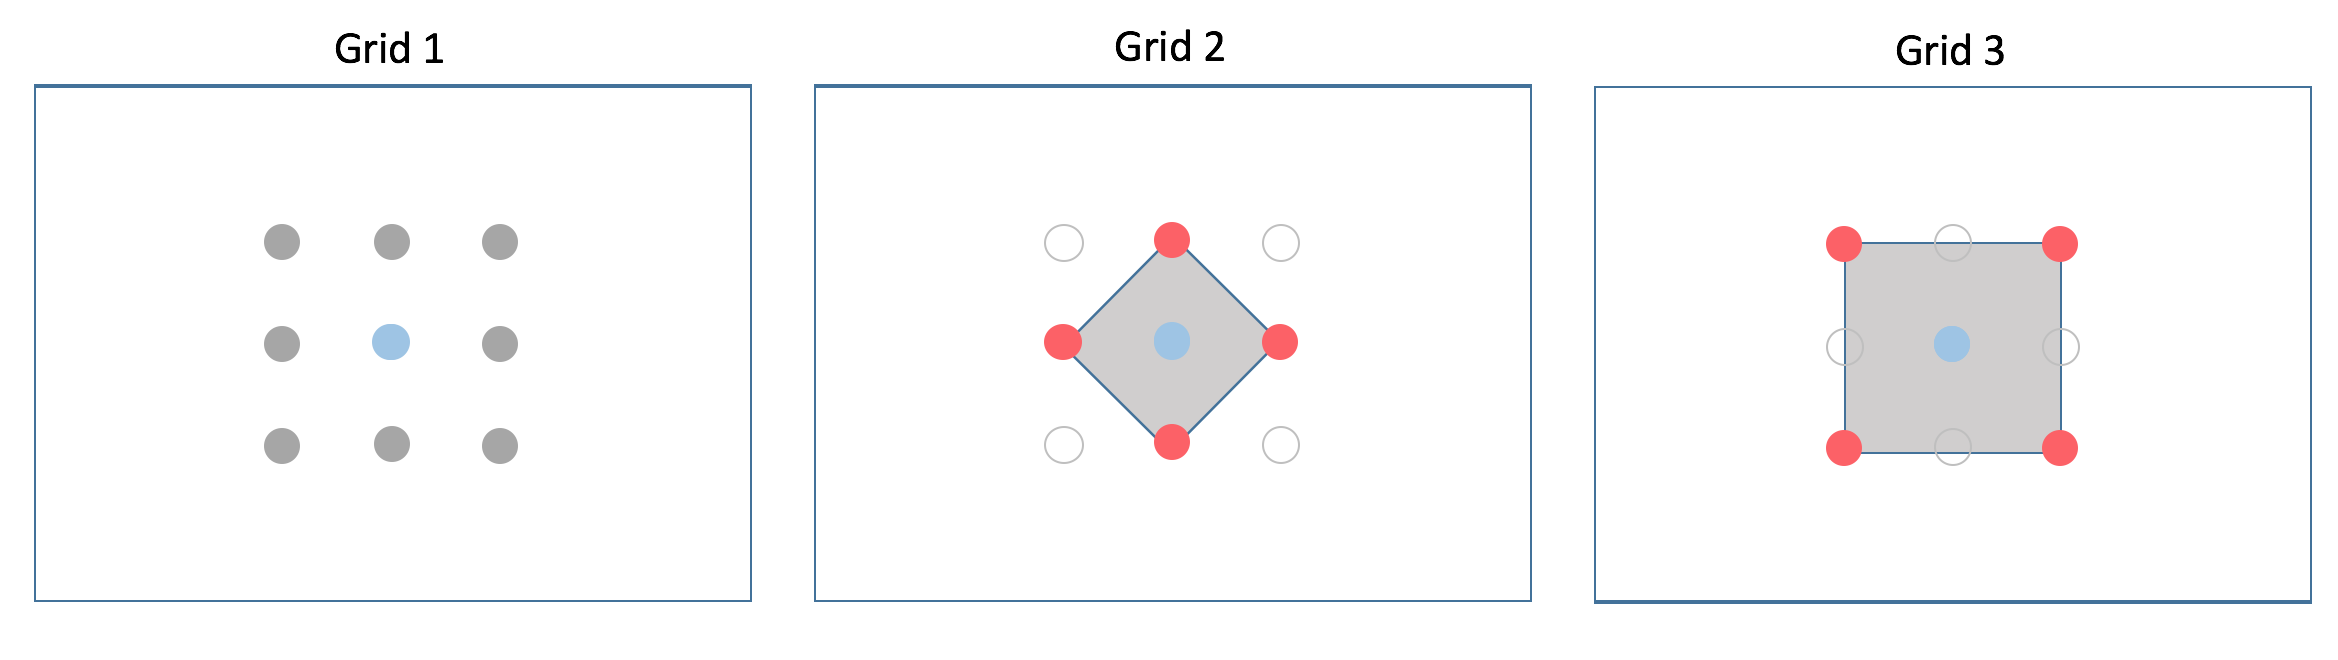
\includegraphics[scale = 0.45]{Sections/FurtherWork/images/grids2.png}}
				\caption{Illustration of how the grid of \ac{RIR} positions used for interpolation could be simplified in an attempt to speed up the system. \textbf{Grid 1} shows the layout of the original grid used. \textbf{Grid 2} shows a layout where only the \ac{RIR} locations at 90 degree angles to the user are available reducing the area in which the user can move (shown by the grey square). \textbf{Grid 3} uses \ac{RIR} locations at diagonals to the user increasing the area available but decreasing accuracy.}
				\label{grids}
			\end{figure}

	\subsection{Accuracy}
		\subsubsection{RIR Modelling}
			As mentioned in \nameref{background:aims}, using the direct \ac{RIR} rendering method allows for the calculation of \ac{RIR}'s offline. This lends itself to the potential of using \ac{RIR}'s calculated using the more accurate, but computationally expensive wave-based methods. Using methods discussed in \cite{Southern}, it is possible to combine the accurate low frequency models with the much less computationally expensive high frequency accurate models calculated using geometrical acoustic modelling methods used in Odeon. If this were done, it would be interesting to re-run user test \#1 to see whether this makes a difference to the perception of distance moved with using the more accurate synthetic \ac{RIR}'s.

		\subsubsection{Surface Materials}
			One issue raised when modelling the room (\nameref{odeon:materials}) was the lack of common materials provided in Odeons material list. This caused issues when trying to produce an \ac{RIR} that more closely resembles the real measurements taken from Hendrix Hall. This could be improved by obtaining more accurate data regarding the rooms interior.

	\subsection{Additional Functionality}
		The original implementation of the \ac{VSS} used an Oculus rift as a head-tracking device and as a means to provide a 360\textdegree~image of the position that the user was placed in. It was decided not to include this feature in this project as it would require obtaining images for each of the \ac{RIR} locations. This would also have had an effect of the perception of mobility as it would not have been possible to convince the user they could move to any location they would like when they can see that they are being placed statically. It would be an interesting extension to include a system that provides the user with a graphical representation of the modelled space in real time, by using the model designed in Google SketchUp and investigating the difference in perception when this feature is active.


	%Could test whether directivity patter when using synthetic RIRs makes a difference

	%Test whether using just a box as a virtual environements makes a difference

	%Include graphics


	% Obtaining better surface material information to further improve the accuracy of the synthetic RIRs


\end{document}